\begin{chapter}{Force Field Development Workflow}

\begin{figure}
\centering
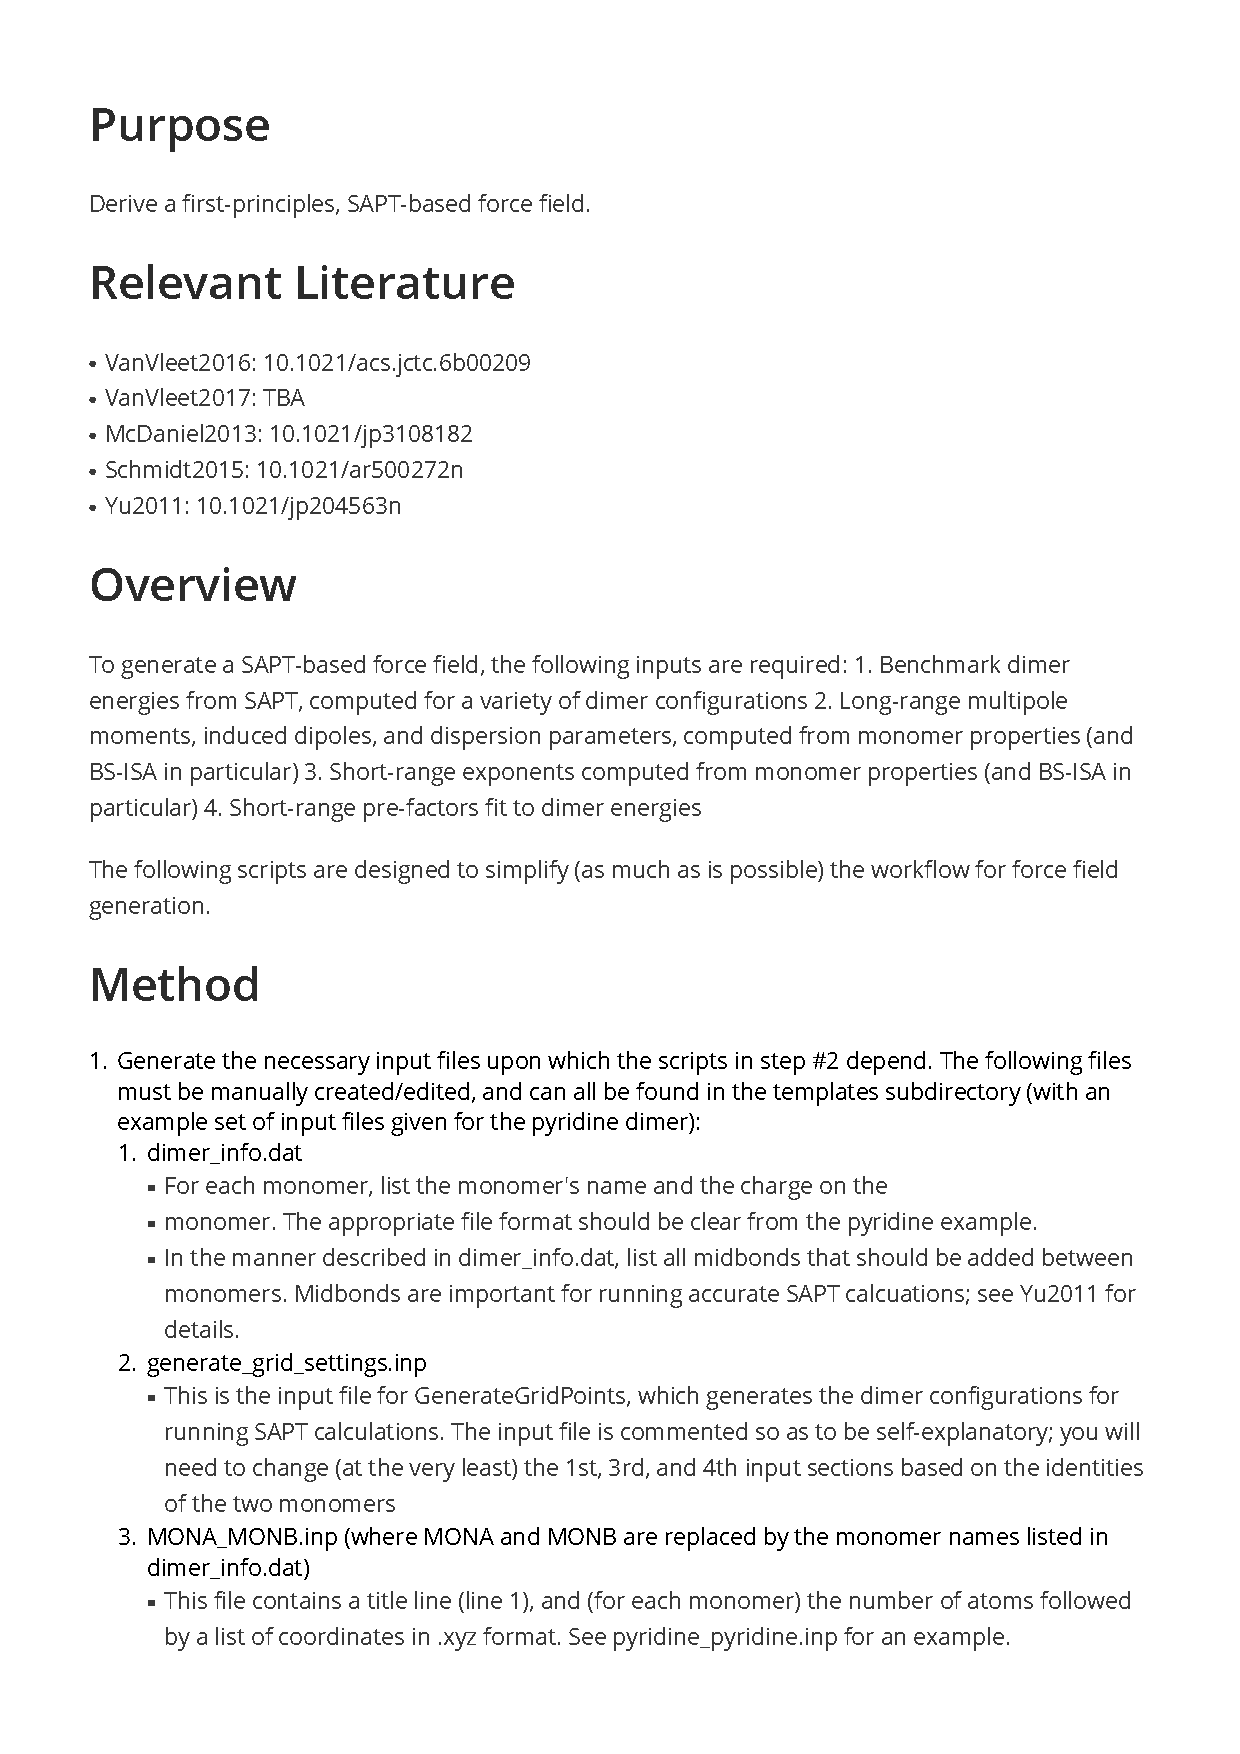
\includegraphics[page=1,width=1.0\textwidth]{workflow/github_readme.pdf}
%\caption[GitHub Overview for FF Workflow]{Workflow 1!}
\phantomcaption
\end{figure}
\begin{figure}\ContinuedFloat
\centering
\includegraphics[page=2,width=1.0\textwidth]{workflow/github_readme.pdf}
%\caption[GitHub Overview for FF Workflow]{Workflow 2!}
\phantomcaption
\end{figure}
\begin{figure}\ContinuedFloat
\centering
\includegraphics[page=3,width=1.0\textwidth]{workflow/github_readme.pdf}
\caption[The Semi-Automated Workflow for Force Field Development]{An overview
of the semi-automated force field
development process. The full workflow and required scripts can be found at
\url{https://github.com/mvanvleet/workflow-for-force-fields}.}
%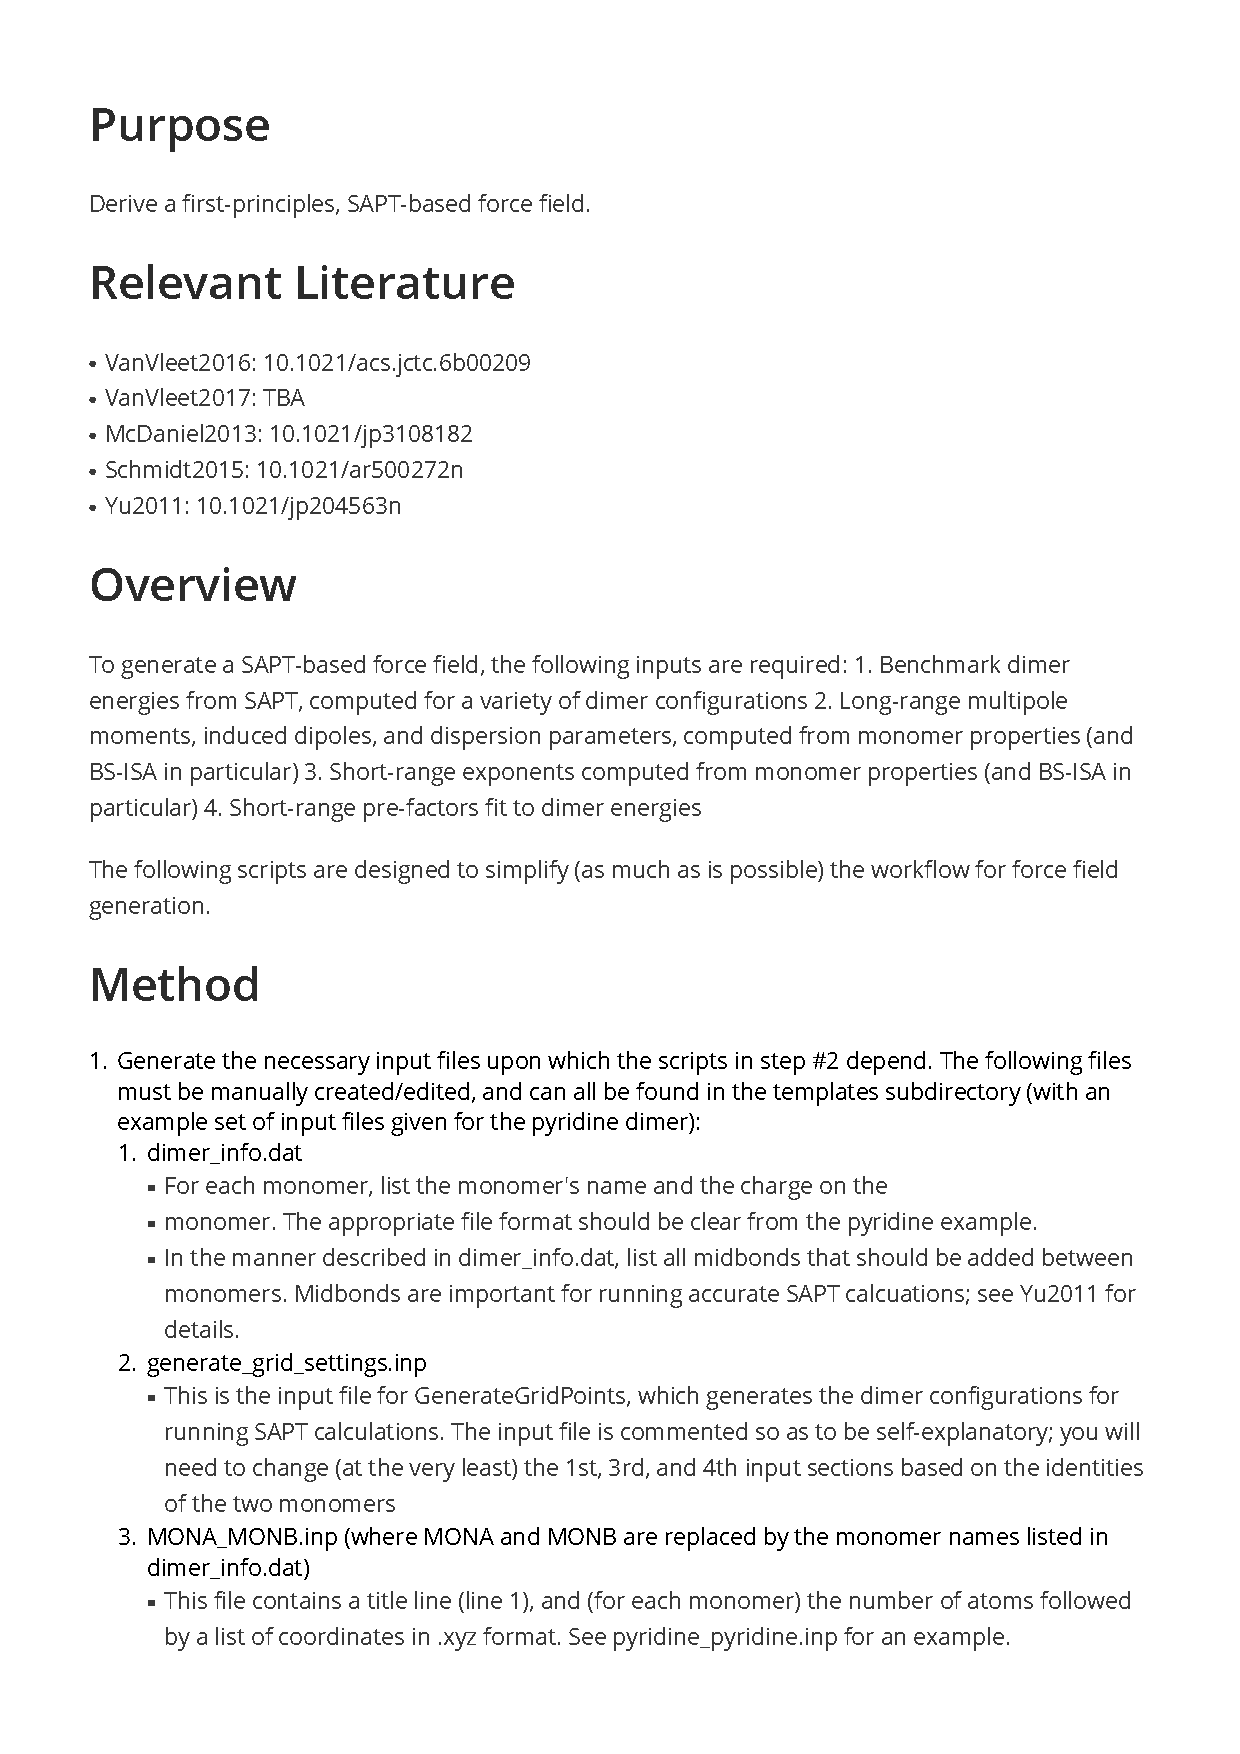
\includepdf[pages={1-},scale=0.75]{workflow/github_readme.pdf}
\label{fig:workflow-overview}
\end{figure}

\end{chapter}

\clearpage

